\section{Wideband Spectrum Sensing}
This section presents a new method of sensing sparse signals, and its application to the problem of sensing over wideband spectra in Cognitive Radios. Initially we introduce Classical Sensing and then give an overview of both Compressive Sensing and Group Testing. Finally, we discuss some sub-Nyquist sampling techniques.

\begin{figure*}[h]
\centering
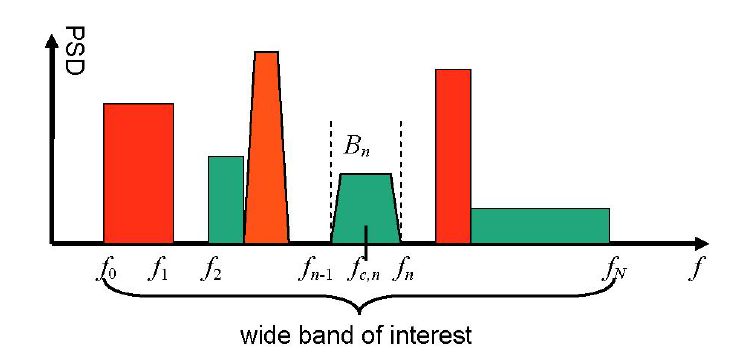
\includegraphics[height = 7 cm]{bands.png}
\caption{A digram of the Spectrum Sensing model \cite{Tian}}
\label{widebandspectra}
\end{figure*}



\subsection{Compressed Sensing}

However, in practice many signals encountered 'in the wild' can be fully specified by much fewer bits than required by the sampling theorem above. For example, image compression algorithms can reduce the size of a stored image to about 1\% of the size required by Nyquist sampling. If the reconstruction algorithm is able to reconstruct the image from this small amount of data, this raises the question: why collect all the data in the first place, when most of the information can be thrown away? Why not directly measure the part that will not end up being thrown away?

Compressed Sensing considers situations where the signal is \textit{undersampled} i.e. situations in which the number of samples is much smaller than the dimension of the signal (or the number of samples required by classical sampling theory). This is equivalent to a system of linear equations which is under-determined.  That is, this is a method of measuring the informative parts of a signal directly without acquiring unessential information at the same time (i.e. the parts of the signal that would be discarded in traditional compression applications). The questions then are how can we acquire these measurements in the first place, and how to 'decompress' them once they are obtained \cite{Donoho2006}. 

To answer the first, note that signals have representations in which they are sparse (i.e. the most of the co-efficients in that representation are zero, or close to zero). For example, 

\begin{enumerate}
\item  A sine wave at frequency \(\omega\) is defined as a single spike in the frequency domain yet has an infinite support in the time domain
\item An image will have values for every pixel, yet the wavelet decomposition of the image will typically only have a few non-zero coefficients
\end{enumerate} 

However, we may not be able to directly obtain those coefficients, as we may not posses an appropriate measuring device (or one may not exist). Yet we are able to measure correlations between the signal and the basis waveforms of the domain where the signal is sparse \(\phi_{k}\) i.e. 
%
\begin{equation}
y_{k} = \left\langle f \text{,} \phi_{k} \right\rangle \text{ } k = 1 \ldots m
\end{equation}
%
for \( f \in \mathbb{R}^n \) expanded in an orthonormal basis \( \psi \) s.t.
%
\begin{equation}
f(t) = \sum_{i = 1}^n x_{i}\psi_{i}(t) 
\end{equation}
%
where the \(x_{i} \) are the coefficient sequence of f. 

An example of a practical Compressive Sensing system is the single-pixel camera at Rice University \cite{Duarte2008}, \cite{wakin2006architecture}. Typical camera devices obtain pixel samples by exposing a bank of photon detectors (one for each pixel) to the incident light field. This data is the processed into an image.

The single pixel camera takes pictures by first directing the incoming light field onto an array of tiny mirrors (one for each pixel). Each mirror can be either be oriented towards a single photon detector, or oriented away from the detector. In this setup, a measurement is taken as the sum of all the incident light beams. Afterwards, the mirrors are flipped to a new random configuration, and another measurement is taken. This process is repeated, until enough information has been collected to reconstruct the image. Figure \ref{singlepixelcamera} shows the operation of the single pixel camera.

\begin{figure*}[h]
\centering
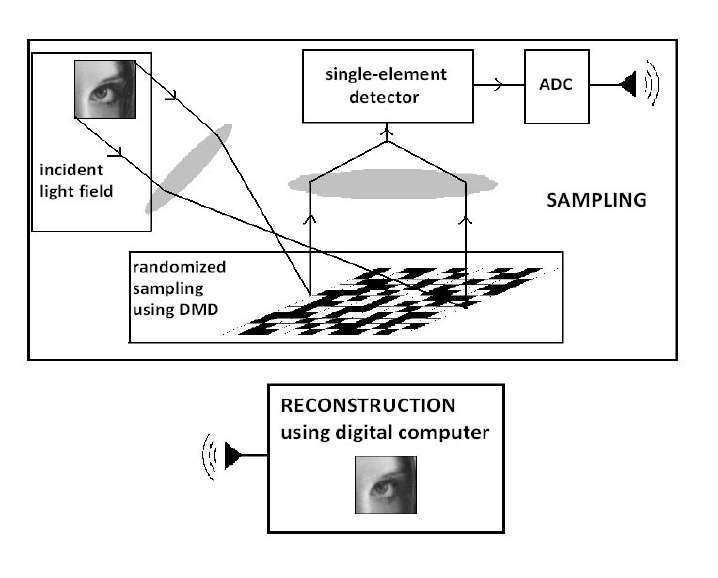
\includegraphics[height = 7 cm]{singlepixel.png}
\caption{The operation of the single pixel camera at Rice University \cite{Thompson2011}, \cite{DavenportSinglePixel}}
\label{singlepixelcamera}
\end{figure*}

%Compressive Sensing works best if the \(x_{i}\) are compressible (i.e. they are distributed according to a power law), and the error \(\|x - x_{s}\|\) is small.

%In Compressive Sensing measurements are taken is an incoherent basis, as opposed to the basis of the original signal. 

The question all this raises is where do we do our sensing? In other words, given that we know a basis in which our signal is sparse, \(\phi\), how do we choose \(\psi\)? It's best to choose \(\psi\) so that the signal is 'spread out' relative to the signal's expansion in \(\phi\). Such pairs are said to be incoherent. 

\begin{defn}
A pair of bases is said to be incoherent if the largest projection of two elements between the sensing (\(\psi\)) and representation (\(\phi\)) basis  is in the set \( [1 , \sqrt{n}] \), where \( n \) is the dimension of the signal. The coherence of a pair of bases is denoted by \(\mu\).
\end{defn}

This implies that sensing with incoherent systems is good (in the sine wave example above it would be better to sample randomly in the time domain as opposed to the frequency domain), and efficient mechanisms ought to acquire correlations with random waveforms (e.g. white noise).

\textbf{Theorem} \cite{Candes2006}
Fix f \(\in \mathbb{R}^n\) with a sparse coefficient basis, \(x_{i}\) in \(\psi\). Then a reconstruction from \(m\) random measurements in \(\phi\) is possible with probability \(1 - \delta\) if: 

\begin{equation}
m \geq C \mu^2(\phi, \psi) S \log\left(\frac{n}{\delta}\right)
\end{equation}
\label{minsamples}

where \( \mu(\phi, \psi)\) is the coherence of the two bases, and \(S\) is the number of non-zero entries on the support of the signal.

Then \(f*\) (the proposed reconstruction) is given by \(f^* = \psi x^*\) where \(x^*\) is the solutionn to the convex optimisation program (n.b. \(\| x\|_{l_{1}} := \sum_{i} |x_{i}| \)):

\begin{equation}
min\|\tilde{x}\|_{l_{1}} \text{ subject to } y_{k} = \left\langle \phi_{k} \text{,} \psi x^* \right\rangle \text{   } \forall k \in M \subset [1 \ldots n]
\end{equation}
\label{program0}

i.e. \textbf{CS: Sample non-adaptively in an incoherent domain and invoke linear programming after the acquisition step}

Thus the role of \(l_{1}\) minimisation is to decompress the data. There are many ways to perform this operation: some popular methods are basis pursuit \cite{Chen1998} and Greedy approaches such as Orthogonal Matching Pursuit \cite{Tropp2007}. 

It may be remarked that the \(l_0\) norm:
%
\begin{equation}
\vectornorm{l_0} = \{\# i, x_i \neq 0\}
\end{equation}
%
is a more appropriate functional to minimise. In fact under this norm, \(m \geq 2k\) measurements will suffice to uniquely determine all \(k\)-sparse signals. However, this norm is not convex and so minimising it is an NP-hard problem. As we are seeking sparse solutions the \(l_1\)-norm will suffice \cite{Donoho2006a}. This is because all vectors in a random \(k\)-dimensional subspace of an \(n\)-dimensional space are approximately Gaussian (in the sense that the components are distributed according to an approximate normal distribution). Such vectors have roughly equivalent norms, and so any solution to the \(l_1\) minimisation problem will be the same solution to the \(l_1\) minimisation problem for sufficiently sparse signals.

\subsubsection{Incoherence, isometries and all that}
To recover a sparse vector, we must make sure that the vectors are not in the null space of the sensing matrix (otherwise there would be no hope of recovery). We also require that any subset of \(S\) columns taken from the measurement matrix be nearly orthogonal w.r.t sparse vectors: i.e. all pairwise distances between S-sparse vecotrs be well preserved in the measurement space.

This can be summed up in the following inequality (Restricted Isometry Property) \cite{Emma}:


\begin{definition}[Restricted Isometry Property]
\begin{equation}
\left(1-\delta\right)\vectornorm{x}_{l_2}^2 \leq \vectornorm{Ax}_{l_2}^2 \leq \left(1+\delta\right) \vectornorm{x}_{l_2}^2
\end{equation}
\label{RIP}
\end{definition}

Note, that the RIP isn't necessary for a complete theory of Compressive Sensing, \cite{candes2011probabilistic}, it's however a handy tool for analysing the performance of CS in a variety of situations. This is not the only fomrulation of the RIP possible, for a more comprehensive overview see \cite{foucart2013mathematical}.

We are also in a position to evaluate the meaning of the constant \(\mu\) in \ref{minsamples}. We are considering sampling within orthonormal systems (for example, Time and Frequency):
%
\begin{equation}
A*A = nI
\end{equation}
\label{orthonormal}
%
so that each row or column has \(l_2\) norm equal to \(sqrt{n}\). \(A\) is any matrix satisfying this property (examples include the Fourier matrix and the Dirac matrix). Thus \(\mu\) must be in the set \(\left[1, \sqrt{n}\right]\). \(\mu\) then, is a measure of how concentrated the rows of our measurement matrix is - i.e. how much information is spread across each vector. If \(\mu = 1\) then the rows are 'flat' -  and we need relatively fewer samples to reconstruct an S-sparse signal (i.e. each sample provides the same amount of information). However, if the rows contain all non-zero entries except for a single component, then \(\mu^2 = n\) and we will need to observe all components to determine the non-zero one (i.e. we have no guarantees of recovery from limited samples) \cite{Candes2007}. 

Noting that the measurements we take are projections from our orthonormal system (from example time) onto a sparsifying basis (i.e. frequency) we can see that:

\begin{equation}
\mu = max_{k,j} |\langle \phi_k, \psi_j \rangle |
\end{equation}
\label {mudef}
 
So we need to choose a sensing basis, where the vectors will be 'spread out', and the degree of spreading is characterised by \(\mu\).

\subsubsection{Short, Fat matrices}
As remarked upon earlier: Compressive Sensing is equivalent to solving an under-determined linear system, with the constraint that we seek the sparsest solution. The content of the previous sections amounts to constraints on the number of rows of matrix of this linear system. 

If we had an Oracle which could tell us where the non-zero components of our solution were, then we would need only as many rows of the matrix as there were non-zero components in the signal to fully specify the problem. 

%\begin{figure*}[h]
%\centering
%\includegraphics[height = 7 cm, width=\textwidth]%{compressive_sensing_example.jpg}
%\caption{A visualisation of the Compressive Sensing problem as an under-%determined system}
%\label{l1l2}
%\end{figure*}

However, such and Oracle does not exist, and so we're left with the task of constructing a matrix to recover those components. Knowing that we're looking for k-sparse solutions, we need a matrix with at least 2k columns which are linearly independent. Equivalently, all images of \(k\)-sparse vectors under the operation of the sensing matrix \(\Phi\) must be distinct. From this, any k-sparse signal can be reconstructed from \(Ax\). 

To prove this assume the opposite - then there are two vectors \(x, x' \in \mathbb{R}^n\) such that \(Ax = Ax'\). I.e. \(A(x-x') = 0\). However, \((x-x')\) is 2k-sparse and so there is a linear dependence between 2k columns of the sensing matrix A. We have a contradiction, and so 2k columns will suffice to reconstruct a k-sparse signal. 

The problem with this is that we are trying to find the support of a k-sparse signal over a vector of length N, and so we would need to check all \(N \choose k\) combinations of k-sparse signals which is prohibitively computationally expensive. Is there some way to gain the advantages of sparsity, without having to minimise a non-convex functional?

As it turns out, the answer is yes. If we take \( m \geq C \mu^2(\phi, \psi) S \log\left(n\right) \) rows minimising the \(l_{1}\) norm will find the sparsest solution. This is because the \(l_1\) norm is an octahedron (in 3-dimensions, in higher dimensions it has an analogous spiky geometry), and solutions are more likely to intersect the norm at the points. Figure \ref{l1l2} shows this.

\begin{figure*}[h]
\centering
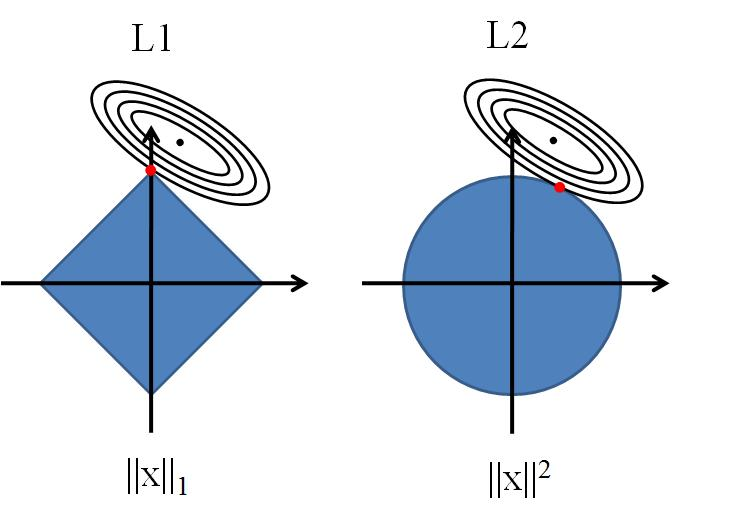
\includegraphics[height = 7 cm]{l1l2.jpg}
\caption{Solutions to the Compressive Sensing optimisation problem intersect the \(l_1\) norm the points where all components (but one) of the vector are zero (i.e. it is sparsity promoting) \cite{Tibshirani1996}}
\label{l1l2}
\end{figure*}

\subsection{Reconstruction Algorithms}
Compressive sensing places the computational load on reconstructing the Nyquist samples \(x\), from the set of compressive samples \(y\). There are many reconstruction algorithms, which fall into three broad classes: convex-optimisations/linear programming, greedy methods, and Bayesian statistical methods (discussed in detail in section \ref{sec:BayesianCS}). Convex optimisation methods offer better performance at the cost of greater computational complexity. Greedy methods are relatively simpler, but don't have the performance of convex algorithms. A recent greedy method, Approximate Message Passing (AMP), is a blend of both \cite{donoho2009message}.

Convex algorithms all relax the \(l\)-0 requirement for recovery \cite{tropp2006relax}, by instead solving the equivalent \(l\)-1 minimisation problem:

\begin{equation}
\argmin_x \vectornorm{x}_1 \text{ s.t } y=Ax
\end{equation}

in the noiseless case, and 

\begin{equation}
\argmin_x \frac{1}{2}\vectornorm{Ax-y}_2^2 + \lambda\vectornorm{x}_1
\end{equation}

in the noisy case.

The representative algorithm for this type of minimisation is Basis-Pursuit \cite{Chen1998a}. 

Candes and Tao in \cite{candes2007dantzig}, propose an algorithm based on the following functional:


%There has been a line of work on algorithms directly minimising the \(l\)-0 norm \cite{wen2015efficient}, \cite{oxvig2012improving}, \cite{mohimani2010sparse}.

Greedy methods and iterative shrinkage algorithms, are another family of solutions to \ref{program0}. They offer reduced computational complexity with correspondingly worse reconstruction quality and poorer guarantees on sparsity and undersampling than convex algorithms. Examples of this type are Orthogonal Matching Pursuit (OMP)\cite{tropp2007signal} and Iterative Thresholding (IT) \cite{blumensath2009iterative}, \cite{Beck2009}. 

The Greedy family of algorithms abandons exhaustive searches of the solution space in favour of locally optimal single term updates. They proceed by approximating the solution by some active set of columns from the sensinng matrix \(A\) and solving a restricted least-squares problem at each (in the case of OMP). This guarantees a maximal reduction in \(l\)-2 error in each iteration.

However, due to their greedy nature, these algorithms are not guaranteed to converge: in fact it can be shown that there exist \(k\)-sparse vectors and sensing matrices \(A\) such that OMP fails to converge in k iterations \cite{wen2013improved}.

Iterative shrinkage algorithms are similar to greedy algorithms, but replace the single term updates by a iteratively denoised gradient descent. The choice of the (component-wise) denoiser is dependent upon the regulaiser used in \ref{program0}. These algorithms have an interpretation as Expectation-Maximisation \cite{figueiredo2003algorithm} - where the E-step is performed as gradient descent, and the M-step is the application of the denoiser.

Belief propagation (BP) \cite{Yedidia2011} is a popular iterative algorithm, offering improved reconstruction quality and undersampling performance. However, it is a computationally complex algorithm. It is also difficult to implement. Approximate message passing solves this issue by blending BP and (IT).

The algorithm proceeds like iterative thresholding, but computes an adjusted residual at each stage. The extra term comes from a first order approximation to the messages passed by BP \cite{metzler2014denoising}.

\subsubsection{Bayesian Compressive Sensing}
\label{sec:BayesianCS}
Based on the discussion above we can represent the compressive sensing measurements as: 

\begin{equation}
\textbf{g} = \Phi	\textbf{w}
\end{equation}

where \(\Phi\) is a \(K \times	N\) matrix which is the product of the measurement and sparse bases described earlier.

Note that the measurements may be noisy, with the measurement noise represented by a zero mean Gaussian distribution and unknown variance \( \sigma^2 \):

\begin{equation}
\textbf{g} = \Phi \textbf{w} + \textbf{n}
\end{equation}
\label{CSequation}

Where \textbf{n} is the vector representing the vector of noise, and has the same support as the measurements. 

Previous sections have shown how the weights \(w\) may be found through optimisation methods such as basis pursuit or greedy algorithms. Here, an alternative Bayesian model is described.

From \ref{CSequation} we have a Gaussian likelihood model: 

\begin{equation}
p \left( \textbf{g} \mid \textbf{w}\text{,} \sigma^2 \right) = (2 \pi \sigma^2)^{-K/2} \exp{\left(- \frac{1}{2 \sigma^2} \|\textbf{g} - \Phi	\textbf{w}\|_{2}^{2} \right)} 
\end{equation}

The above has converted the CS problem of inverting sparse weight \textbf{w} into a linear regression problem with a constraint (prior) that \textbf{w} is sparse. 

To seek the full posterior distribution over \textbf{w} and \( \sigma^2 \), we can chose a sparsity promoting prior. A popular sparseness prior is the Laplace density functions:

\begin{equation}
p\left(w\mid\lambda\right) = \left(\frac{\lambda}{2}\right)^N exp{-\lambda \sum_{i=1}^{N} |w_i|}
\end{equation}

Note that the solution the convex optimisation problem \ref{program0} corresponds to a maximum \textit{a posteriori} estimate for \(w\) using this prior. I.e this prior is equivalent to using the \(l_1\) norm as an optimisation function (see figure \ref{laplacenormal} \cite{Tibshirani1996}).

\begin{figure*}[h]
\centering
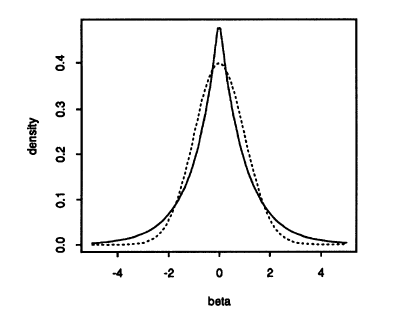
\includegraphics[height = 7 cm]{LaplaceandNormalDensity.png}
\caption{The Laplace (\(l_1\)-norm, bold line) and Normal (\(l_2\)-norm, dotted line) densities. Note that the Laplace density is sparsity promoting as it penalises solutions away from zero more than the Gaussian density. \cite{Tibshirani1996}}
\label{laplacenormal}
\end{figure*}

The full posterior distribution on \(w\) and \(\sigma^2\) may be realised, by using a hierarchical prior instead. To do this, define a zero-mean Gaussian prior on each element of \(w\):
%
\begin{equation}
p\left(w\mid a\right) = \prod_{i=1}^{N}\mathbb{N}\left(w_i\mid 0, \alpha_{i}^-1\right)
\end{equation}
%
where \(\alpha\) is the precision of the distribution. A gamma prior is then imposed on \(\alpha\):

\begin{equation}
p\left(\alpha \mid a, b \right) = \prod_{i=1}^{N} \Gamma\left( \alpha_i \mid a, b \right)
\end{equation}

The overall prior is found by marginalising over the hyperparameters:

\begin{equation}
p\left( w \mid a, b \right) = \prod_{i=1}^{N} \int_{0}^{\infty} \mathbb{N}\left(w_i\mid 0, \alpha_{i}^-1\right) \Gamma\left( \alpha_i \mid a, b \right)
\end{equation}

This integral can be done analytically and is a Student-t distribution. Choosing the parameters \(a,b\) appropriately we can make the Student-t distribution peak strongly around \(w_i = 0\) i.e. sparsifying. This process can be repeated for the noise variance \(\sigma^2\). The hierarchical model for this process is shown in \ref{bayesiancs}. This model, and other CS models which not necessarily have closed form solutions, can be solved via belief-propagation \cite{Baron2010}

\begin{figure*}[h]
\centering
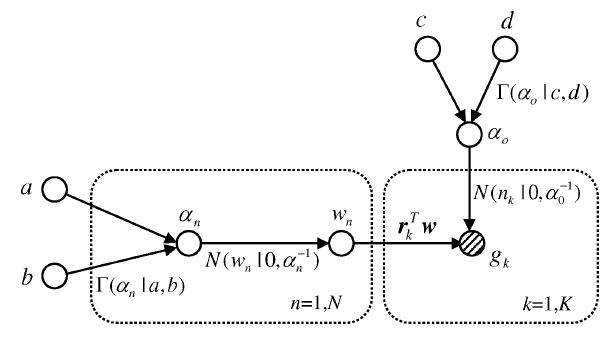
\includegraphics[height = 7 cm]{bayesiancs.png}
\caption{The hierarchical model for the Bayesian CS formulation \cite{Ji2008}}
\label{bayesiancs}
\end{figure*}